This section will describe how we used the project backlog as well as how we handled each sprint. \\

The backlog can be seen in \autoref{fig:projectBacklog}. \\

Our backlog consists of: 
\begin{itemize}
\item An ID for the assignment
\item A name 
\item A priority from 1-10, 1 being the highest
\item An estimate of the time taken
\item A ``how to demo'' description
\item A possible note
\item A status 	
\end{itemize}
Note that time taken is not actual hours but a relative value. This means that an assignment with the value 4 should take twice as long as an assignment with the value 2, but not necessarily take 4 and 2 hours respectively.

The project backlog is divided into colors. The colors represent during which sprint the assignment was added starting with before sprint 1, during sprint 1, before sprint 2, during sprints 2 etc. The status attribute has 4 values: Not started, Completed, Waiting for external source, and In progress

The project backlog was a new tool for us this semester, therefore we had some troubles or misunderstandings in the start of the project, that we sorted out in the end. The two biggest problems we encountered was the estimation of time and vaguely defined assignments. 

Our first version of the backlog was short and unspecific. The result of this was that or assignments were large and it was hard to estimate the time it would take. Also we felt like no progress was happening because we did not finish a lot of the assignments during a sprint. To counter act that, we started splitting our assignments into smaller more concrete assignments. This made it easier for us to estimate the time and we started to finish more assignments during a sprint giving a feeling of progress. 

An example of this is the web interface, first it was defined as two tasks called GUI design and CRUD management. These two assignments covers the whole web interface part of our project which is roughly 33 \%. Even though we gave them a big time estimate of 20 and 10 respectivly this was nowhere near enough time to finish it. These two assignments kept being in the ``in progress'' state for quite some time. After that we decided to split the two assignment into much more concrete assigments. This resultet in 20 much more managable assignments like ``add a profile'' or ``delete a tag''. 

Our sprints reflects this progress of experience as well

\begin{description}
\item [Sprint 1, from ? to ?]
	During this sprint we focused on the Database and the sw6ml schema. We wanted to start out light because we had no idea how much we where capable of doing during one sprint, so we decided that it was better to put too little on the sprint backlog and then add on some assignments if necessary than to put too much on the sprint backlog and struggle to finish it. We found that we could easily finish what we had decided, but this was mainly because we had done a lot of work prior to the sprint so much of the work was already done.
\item[Sprint 2, from 26/03/2012 to 04/04/2012]
	During this sprint we started working on the design of the web interface. We also had to update the sw6ml schema and the database to new requirements as well as looking into auto generation of primary keys and incrementation of IDs. Server data I/O and transmission packages was also worked on in this sprint. In the end of the sprint we had a first mock up of our web interface for our contact person so see, therefore we contacted her to schedule a meeting and receive feedback before the beginning of next sprint. The meeting went well and we got some feedback that was added on to our requirements list. 
\item[Sprint 3, from 10/04/2012 to 19/04/2012]
	In this sprint we worked on the CRUD probabilities for the server to communicate with the database. We also had to update the database design and sw6ml schema again to meet new requirements. The server controller which acts as a sort of main class was also planed as well as to create the Savannah data api. On the interface front we only had two assignments: Update the design to meet the requirements received from our contact person during the meeting and implement the web interface on the tomcat. This was where we started to realize that there were much more into the web interface than we thought. This meant that we did not finish anything web interface related
\item [Sprint 4, from 23/04/2012 to 02/05/2012]
	In this sprint we had added a lot of assignment to the project backlog that were transfered to the sprint backlog. This sprint backlog was unlike the three others in that it had almost trice as many assignments than earlier. This was because of the assignment reworking. All the assignments where smaller and much more manageable so even though there where trice as many assignments we also finished trice as many assignments during the sprint.
\item[remaining sprints]
	Sprint 4 became our last ``normal'' sprint. The reason for this was that no more assignments where added to the project backlog so we had a clear overview of what needed to be done. We started to focus more on finishing up what we had instead of making new features. This resulted in that we did not utilize the sprint backlog as much as earlier. We started working together with the other groups to make a release and to plan out our usability test which was carried out in sprint 6. In this period we also started working on an assignment that has been on our project backlog the whole time -- writing the report.  
\end{description}

\begin{figure}
 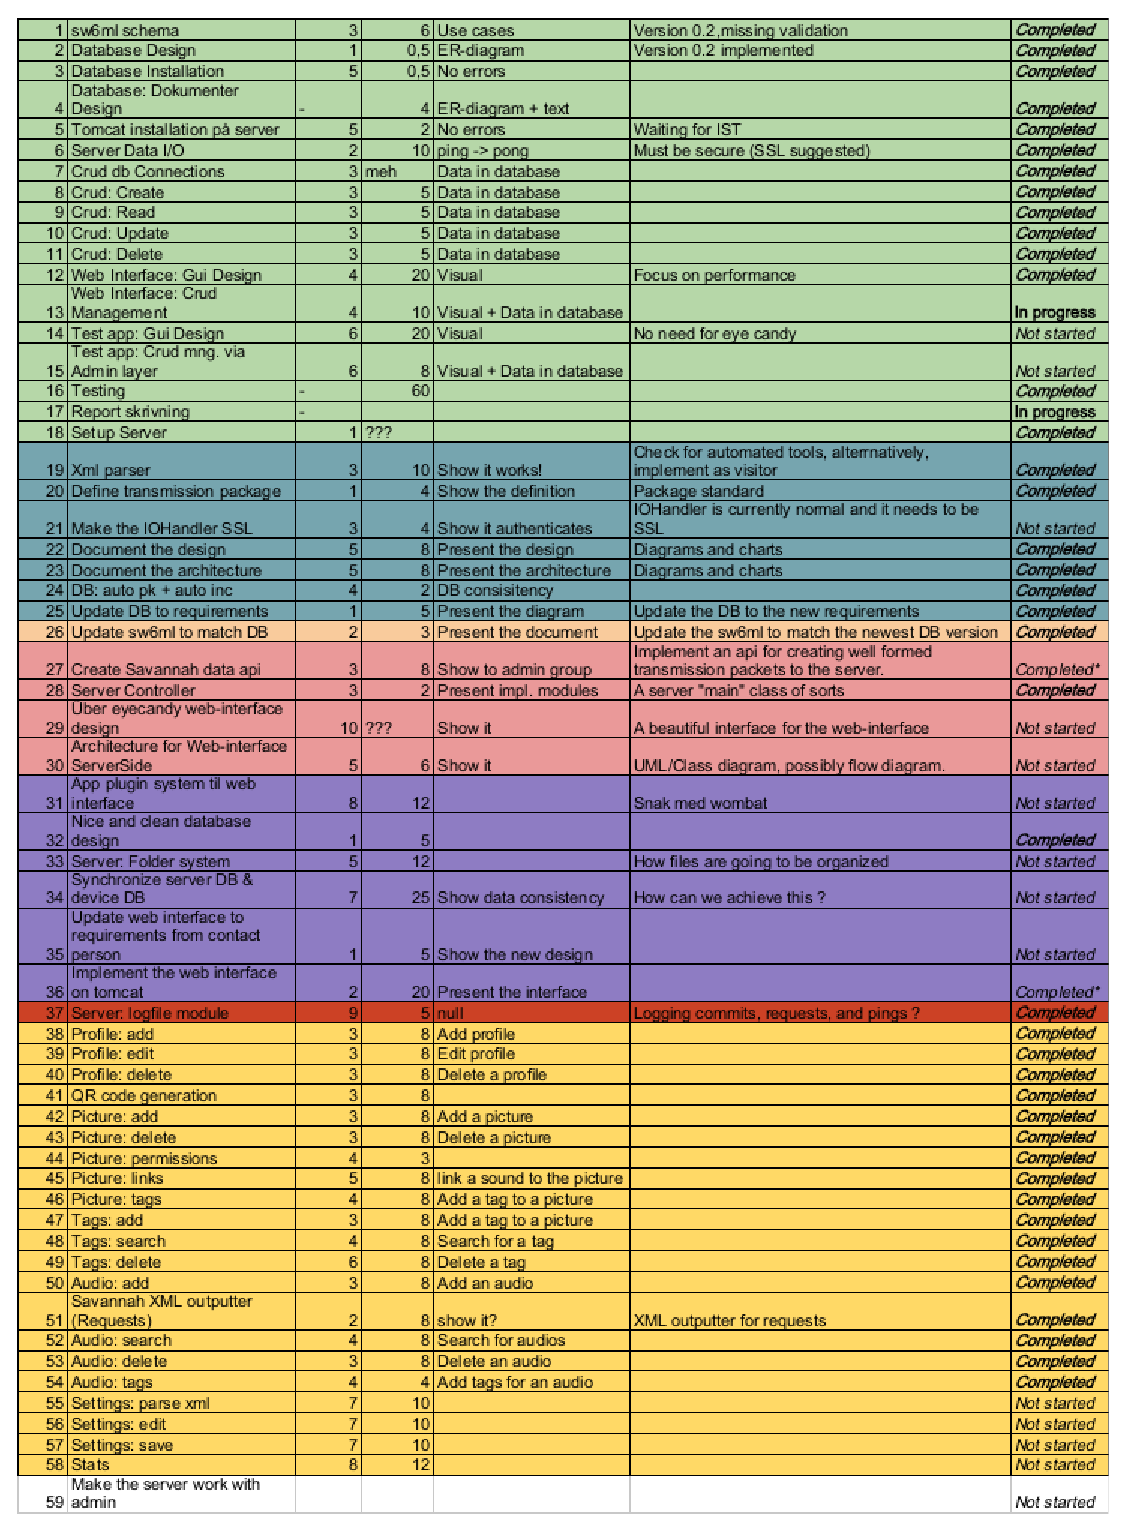
\includegraphics[scale=0.72]{images/projectBacklog}
 \caption{Project backlog.}
 \label{fig:projectBacklog}
\end{figure}

Working in sprints has yield great benefits for the multiproject because all groups have had great knowledge of what other groups where doing and when they could expect certain features to be finished. 